\chapter{Configuration of beam-beam lenses}

\section{Introduction}

The effects of the non-linear forces introduced by beam-beam interactions in the Large Hadron Collider~(LHC) are studied with tracking simulations using, for example, the SixTrack and sixtracklib codes\,\cite{sixtracksite, sixtracklibrepo}. In these simulations the beam-beam interactions are modeled by a set of ``thin'' non-linear lenses around the collision points.
 ``6D beam-beam lenses'' based on Hirata's synchro-beam method\,\cite{hirata, bb6dnote, bb6dslides} are used to model the Head-On (HO) interactions at the for interaction points (IPs) while simpler ``4D lenses'' are used to model parasitic Long-Range encounters\,\cite{casbeambeam}.
 
This document describes a method to configure the beam-beam lenses in tracking simulations based on the MAD-X model of the accelerator, as it has been implemented in the pymask configuration tool\,\cite{masksite}, which has been recently developed as an evolution of existing tools in MAD-X scripting language\,\cite{bbmacrorepo}. In particular, in Sec.\,\ref{sec:posdir}, we discuss how to reconstruct the absolute position of the two beams with respect to the lab frame using the MAD-X twiss and survey tables; in Sec.\,\ref{sec:separ} we discuss how to compute the separation between the two beams; in Sec.\,\ref{sec:xing} we describe how to identify the crossing plane and crossing angle; in Sec.\,\ref{sec:b4} we describe how to configure the anticlockwise beam (conventionally called beam~4)  from the MAD-X model based on two clockwise-oriented sequences; in Sec.\,\ref{sec:crab} we introduce the effect of crab cavities on the beam-beam configuration. 







\section{Identification of the beam position and direction}
\label{sec:posdir}

The position and orientation of the beams at a certain machine element can be obtained from MAD-X combining the information from the survey and twiss tables.

We assume that:
\begin{itemize}
    \item The sequences start from an element at which the reference trajectories of the two beams are known to be parallel;
    \item Both beams (B1 and B2) have the same orientation (clockwise);
    \item Markers or beam-beam lenses are installed at the $s$-locations of the beam-beam interactions.
\end{itemize}

The MAD-X survey provides the coordinates in the lab frame of the two beams:
\begin{equation}
    \textbf{P}^\text{su} = \left(
    \begin{array}{c}
         x^\text{su}\\
         y^\text{su}\\
         s^\text{su}
    \end{array}\right)
\end{equation}
and the corresponding set of angles $(\theta^\text{su}, \phi^\text{su}, \psi^\text{su})$ defining the orientation of the local reference system used by the twiss\,\cite{madsite}. The origin and the orientation of the lab frame are defined by the the first element in the sequence.

The components of the unit vectors defining the local reference frame with respect to the lab frame can be obtained from the following relationship:
\begin{multline}
\left(\hat{\textbf{e}}_x, \hat{\textbf{e}}_y, \hat{\textbf{e}}_s\right)=\\
\left(\begin{array}{ccc}
\cos \theta^\text{su} & 0 & \sin \theta^\text{su} \\
0 & 1 & 0 \\
-\sin \theta^\text{su} & 0 & \cos \theta^\text{su}
\end{array}\right)
\times
\left(\begin{array}{ccc}
1 & 0 & 0 \\
0 & \cos \phi^\text{su} & \sin \phi^\text{su} \\
0 & -\sin \phi^\text{su} & \cos \phi^\text{su}
\end{array}\right)
\times
\left(\begin{array}{ccc}
\cos \psi^\text{su} & -\sin \psi^\text{su} & 0 \\
\sin \psi^\text{su} & \cos \psi^\text{su} & 0 \\
0 & 0 & 1
\end{array}\right)   \, .
\end{multline}

The MAD-X twiss provides the transverse position of the beam in the local reference frame $(x^\text{tw}, y^\text{tw})$, so that the absolute position of the beam in the lab frame can written as
\begin{equation}
    \textbf{P} = \textbf{P}^\text{su} 
    + x^\text{tw} \hat{\textbf{e}}_x
    + y^\text{tw} \hat{\textbf{e}}_y
    \, .
\end{equation}

At the beam-beam locations the local reference frames for the two beams are assumed to be aligned. This is not strictly the case in the regions between the separation-recombination magnets (D1 and D2), but also in that case that case the existing small divergence can be considered negligible.
The beam-beam module of pymask checks the conditions:
\begin{align}
    ||\hat{\textbf{e}}_x^\text{b1} -  \hat{\textbf{e}}_x^\text{b2}|| \ll 1 \, ,\\
    ||\hat{\textbf{e}}_y^\text{b1} -  \hat{\textbf{e}}_y^\text{b2}|| \ll 1 \, .
\end{align}
Therefore we will simply define:
\begin{align}
    \hat{\textbf{e}}_x = \hat{\textbf{e}}_x^\text{b1} = \hat{\textbf{e}}_x^\text{b2} \, ,\\
    \hat{\textbf{e}}_y = \hat{\textbf{e}}_y^\text{b1} = \hat{\textbf{e}}_y^\text{b2} \, .
\end{align}

\section{Computation of beam-beam separations}
\label{sec:separ}

The beam-beam separations are defined as the transverse coordinates of the strong beam with respect to the weak beam. They can be computed as:
\begin{align}
    \Delta x &= \hat{\textbf{e}}_x \cdot \left( \textbf{P}^S -  \textbf{P}^W \right) \, ,\\
    \Delta y &= \hat{\textbf{e}}_y \cdot \left( \textbf{P}^S -  \textbf{P}^W \right) \, ,
\end{align}
where the superscripts identify the weak (W) and the strong (S) beam.

Typically the accuracy of the survey table is insufficient to computed the separations correctly, especially for elements that are too far from the first element in the sequence, due to accumulation of errors along the sequence. A correction can be computed looking as the apparent displacement of the closest Interaction Point (IP) between the two surveys, as the IPs are supposed to coincide.

\section{Crossing plane and crossing angle}
\label{sec:xing}

At the beam-beam encounters the local reference frames for the two beams share the same orientation. Therefore the elevation angle $\alpha$ of the crossing plane  and the crossing angle $\theta$ can be computed in the local reference frame, as will be illustrated in the following.



\begin{figure}[t]
\centering
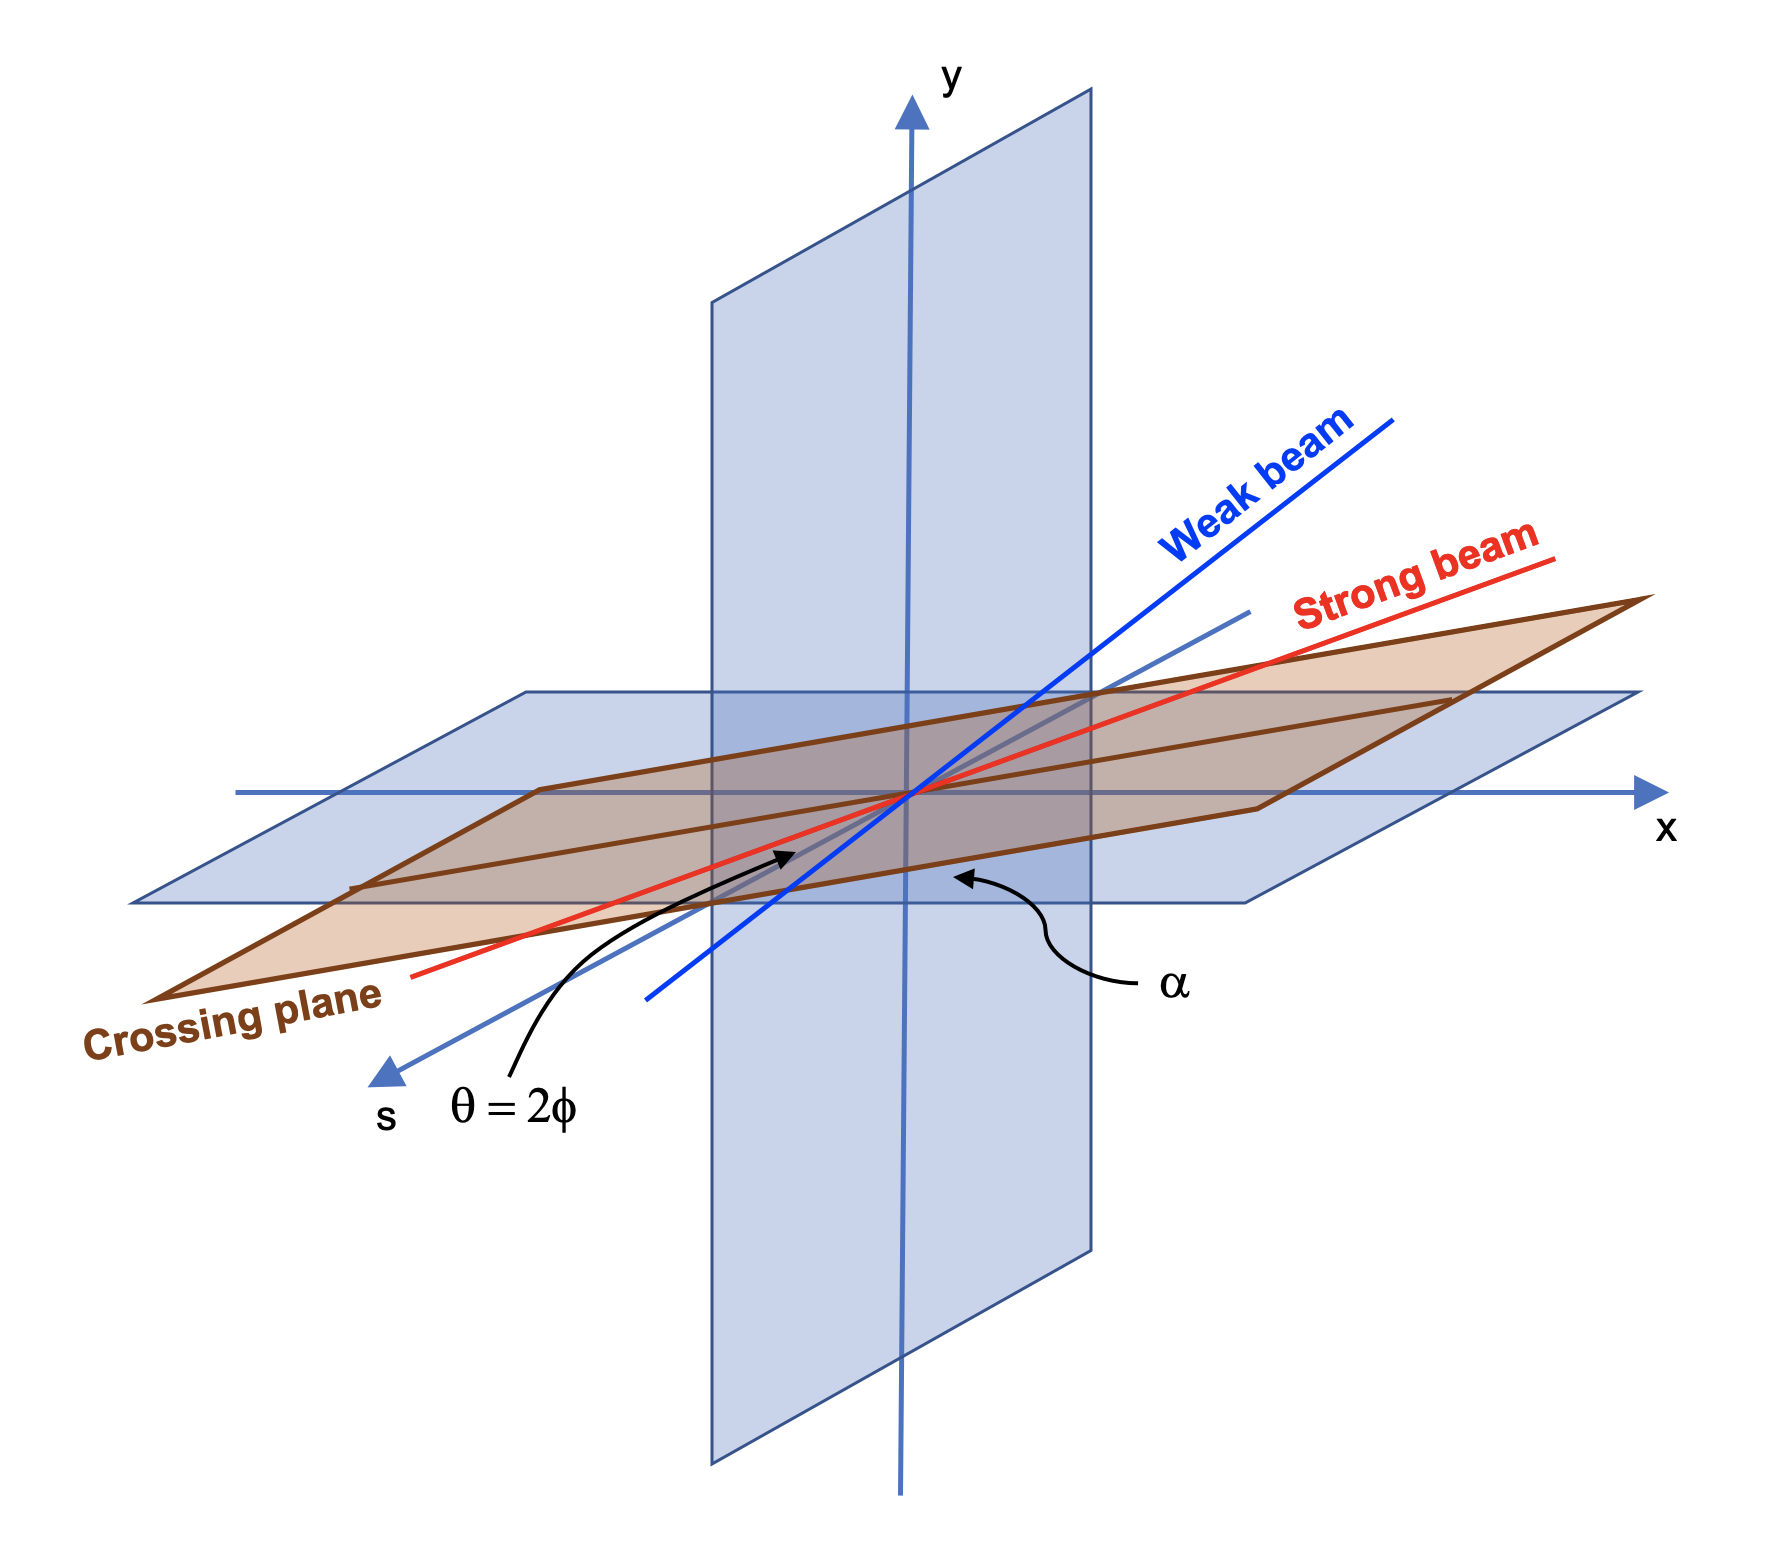
\includegraphics[width=.8\textwidth, trim=0cm 1cm 0cm 1cm, clip]{figures/xang_xplane.png}
\caption{\small Schematic illustration of the crossing plane. \label{fig:xing}}
\end{figure}

\subsection{The crossing plane}

The directions defined by the local trajectories of the two beams are identified by the unit vectors
\begin{align}
\hat{\textbf{p}}^W &= \left(p^W_x, p^W_y, p^W_s\right) \, ,\\
\hat{\textbf{p}}^S &= \left(p^S_x, p^S_y, p^S_s\right) \, ,\
\end{align}
containing the angles of the closed orbit obtained from the twiss of the two beams.

The plane defined by these two directions is called Crossing Plane (XP), as illustrated in Fig.\,\ref{fig:xing}, and its equation is given by:
\begin{equation}
    \textbf{v}_\text{XP}(w_1, w_2) = w_1 \hat{\textbf{p}}^W +
    w_2 \hat{\textbf{p}}^S \, .
\label{eq:xpeq}
\end{equation}

The line defined by the intersection of the crossing plane and the transverse plane identified by the unit vectors $\hat{\textbf{e}}_x$  and $\hat{\textbf{e}}_y$ is given by the condition:
\begin{equation}
\textbf{v}_\text{XP}(w_1, w_2) \cdot \hat{\textbf{e}}_s=0 \, .
\label{eq:inters1}
\end{equation}

Replacing Eq.\,\eqref{eq:xpeq} into Eq.\,\eqref{eq:inters1} we obtain:
\begin{equation}
 w_1 p^W_s + w_2 p^S_s = 0 \, ,
\end{equation}

and replacing this condition in Eq.\,\eqref{eq:xpeq} we obtain the equation of the intersection line
\begin{equation}
    \textbf{v}_\text{T}(w_1) = w_1 \left(\hat{\textbf{p}}^W -
    \frac{p^W_{s}}{p^S_{s}} \hat{\textbf{p}}^S\right)
    \, .
\label{eq:vxy}
\end{equation}



The elevation angle $\alpha$ of the intersection line with respect to the local $x$-direction ($\hat{\textbf{e}}_x$) can be written as:
\begin{equation}
    \alpha=\arctan \frac
    {\textbf{v}_\text{T}\cdot\hat{\textbf{e}}_y}
    {\textbf{v}_\text{T}\cdot\hat{\textbf{e}}_x}
    \, .
\end{equation}

Using Eq.\,\eqref{eq:vxy} we obtain:
\begin{equation}
    \alpha=\arctan \cfrac
    {\left(p_y^W -
    \cfrac{p^W_{s}}{p^S_{s}} p_y^S\right)}
    {\left(p_x^W -
    \cfrac{p^W_{s}}{p^S_{s}} p_x^S\right)}
    \,. 
\end{equation}

In the paraxial approximation ($p^S_{s} \simeq p^W_{s}\simeq 1$) this simply becomes:
\begin{equation}
    \alpha=\arctan \cfrac
    {\Delta p_y}
    {\Delta p_x}
    \, ,
    \label{eq:alpha1}
\end{equation}
where we have defined:
\begin{align}
    \Delta p_x &= p_x^W - p_x^S \, ,\\
    \Delta p_y &= p_y^W - p_y^S \, .
\end{align}
In the legacy beam-beam macros as well as in the configuration pymask tool, the following logic is implemented
\begin{equation}
    \alpha = \begin{cases} 
    \arctan \left(\cfrac
    {\Delta p_y}
    {\Delta p_x}\right) &\mbox{if } \left|\Delta p_x\right| \geq \left|\Delta p_y\right| \\ 
    \cfrac{\pi}{2} - \arctan \left(\cfrac
    {\Delta p_x}
    {\Delta p_y}
    \right)&\mbox{if } \left|\Delta p_x\right| < \left|\Delta p_y\right| \end{cases}
    \, ,
\end{equation}
for which $\alpha$ is limited to the range:
\begin{equation}
     -\cfrac{\pi}{4}  \leq \alpha \leq \cfrac{3}{4}\pi
     \, .
\end{equation}

In particular, for a purely horizontal crossing we have $\alpha=0$ and for a purely vertical crossing we have $\alpha=\frac{\pi}{2}$.

\subsection{The crossing angle}
The crossing angle $\theta$ between the two beams can be found from the relation:
\begin{equation}
\cos\theta=\hat{\textbf{p}}^W\cdot
\hat{\textbf{p}}^S
\, .
\label{eq:dotprod}
\end{equation}

The half crossing angle 
\begin{equation}
    \phi = \frac{\theta}{2}
\end{equation}
is often used instead of $\theta$.

In the paraxial approximation
\begin{align}
    p_x \ll 1 \, ,\\
    p_y \ll 1 \, ,\\
\end{align}
the scalar product in Eq.\,\eqref{eq:dotprod} can be rewritten as
\begin{align}
    \hat{\textbf{p}}^W\cdot
\hat{\textbf{p}}^S &=
p^W_{x}p^S_{x}+p^W_{y}p^S_{y}+p^W_{s}p^S_{s}
\nonumber\\
&= p^W_{x}p^S_{x}+p^W_{y}p^S_{y} +\sqrt{1 - \left(p^W_{x}\right)^2 - \left(p^W_{y}\right)^2}
\sqrt{1 - \left(p^S_{x}\right)^2 - \left(p^S_{y}\right)^2}
\nonumber\\
&\simeq  p^W_{x}p^S_{x}+p^W_{y}p^S_{y}
+\left(1 - \cfrac{\left(p^W_{x}\right)^2}{2} - \cfrac{\left(p^W_{y}\right)^2}{2}\right)
\left(1 - \cfrac{\left(p^S_{x}\right)^2}{2} - \cfrac{\left(p^S_{y}\right)^2}{2}\right)
\nonumber\\
&\simeq p^W_{x}p^S_{x}+p^W_{y}p^S_{y}
+ 1 - \cfrac{\left(p^W_{x}\right)^2}{2} - \cfrac{\left(p^W_{y}\right)^2}{2} - \cfrac{\left(p^S_{x}\right)^2}{2} - \cfrac{\left(p^S_{y}\right)^2}{2}
\, ,
\end{align}
which can be written in compact form as:
\begin{equation}
\hat{\textbf{p}}^W\cdot
\hat{\textbf{p}}^S
\simeq
1 - \cfrac{
\left(p^W_{x} - p^S_{x}\right)^2 + 
\left(p^W_{y} - p^S_{y}\right)^2}{2}
\, .
\label{eq:dotappr}
\end{equation}
For small crossing angle we can write:
\begin{equation}
    \cos \theta \simeq 1-\cfrac{\theta^2}{2} \, .
    \label{eq:cosappr}
\end{equation}
Replacing Eqs.\,\eqref{eq:dotappr} and\,\eqref{eq:cosappr} into Eq.\,\eqref{eq:dotprod} we obtain
\begin{equation}
    \left| \theta \right| = 
    \sqrt{\Delta p_x^2 + \Delta p_y^2} \, .
\end{equation}

The sign of $\theta$ is defined positive when the weak beam needs to rotate in the clockwise sense in the crossing plane in order to be brought on the strong beam. This corresponds to the following sign choices:
\begin{center}
  \begin{tabular}{c|cc}
     &  $\left|\Delta p_x\right| > \left|\Delta p_y\right|$ & $\left|\Delta p_x\right| < \left|\Delta p_y\right|$\\
     \hline
 $\Delta p_x\geq0,\,   \Delta p_y \geq 0$  &$\theta>0$ &$\theta>0$\\
 $\Delta p_x < 0,\,   \Delta p_y \geq 0$  &$\theta<0$ &$\theta>0$\\
 $\Delta p_x < 0,\,   \Delta p_y < 0$  &$\theta<0$ &$\theta<0$\\
 $\Delta p_x\geq0,\,   \Delta p_y < 0$  &$\theta>0$ &$\theta<0$\\
\end{tabular}  
\end{center}
which are consistent with the sign convention used in LHC operation.


\section{Transformations for the counterclockwise beam (B4)}
\label{sec:b4}

The typically used MAD-X model of the LHC consists of two sequences both having clockwise (CW) orientation, conventionally called Beam 1 and Beam 2. To perform tracking simulations of the anticlockwise (ACW) beam, an anticlockwise sequence needs to be generated, which is conventionally called Beam~4. The beam-beam lenses in the Beam~4 sequence can be configured based on the beam-beam lenses defined in Beam~2, taking into account that the two are related by the following change of coordinates:
\begin{align}
    x^\text{ACW} &= -x^\text{CW} \, , \label{eq:b4x}\\
    y^\text{ACW} &= +y^\text{CW} \, , \\
    s^\text{ACW} &= -s^\text{CW} \, .
\end{align}

The corresponding transformation for the transverse momenta is:
\begin{align}
    p_x^\text{ACW} &= +p_x^\text{CW} \, ,\\
    p_y^\text{ACW} &= -p_y^\text{CW} \, .\label{eq:b4py}
\end{align}
This can be easily seen from the fact that:
\begin{align}
    p_x &\simeq \cfrac{dx}{ds} \, ,\\
    p_y &\simeq \cfrac{dy}{ds} \, .
\end{align}

Additionally, from Eqs.\,\eqref{eq:b4x} - \eqref{eq:b4py} it is possible to derive the following relations to transform the $\Sigma$-matrix\,\cite{bb6dnote} of the strong beam:
\begin{align}
    \Sigma_{11}^\text{ACW} &= +\Sigma_{11}^\text{CW} \, ,\\
    \Sigma_{12}^\text{ACW} &= -\Sigma_{12}^\text{CW} \, ,\\
    \Sigma_{13}^\text{ACW} &= -\Sigma_{13}^\text{CW} \, ,\\
    \Sigma_{14}^\text{ACW} &= +\Sigma_{14}^\text{CW} \, ,\\
    \Sigma_{22}^\text{ACW} &= +\Sigma_{22}^\text{CW} \, ,\\
    \Sigma_{23}^\text{ACW} &= +\Sigma_{23}^\text{CW} \, ,\\
    \Sigma_{24}^\text{ACW} &= -\Sigma_{24}^\text{CW} \, ,\\
    \Sigma_{33}^\text{ACW} &= +\Sigma_{33}^\text{CW} \, ,\\
    \Sigma_{34}^\text{ACW} &= -\Sigma_{34}^\text{CW} \, ,\\
    \Sigma_{44}^\text{ACW} &= +\Sigma_{44}^\text{CW} \, .\\
\end{align}



\section{Crab crossing}
\label{sec:crab}

To discuss the effect of crab cavities, we define along the bunches of Beam~1 and Beam~2 (sharing the same $s$ coordinate as in the MAD-X model), the longitudinal coordinates $z_1$ and $z_2$, oriented like $s$.

Assuming that the slices with $z_1 = z_2 = 0$ collide at s=0, the collision point (CP) for two generic slices $z_1$ and $z_2$ is at the location:
\begin{equation}
    s_\text{CP} = \frac{z_1 + z_2}{2} \, .
    \label{eq:cp}
\end{equation}

In the absence of crab crossing, the transverse position of the two beams is independent from $z$:
\begin{align}
    x_1 &= +\phi s \, ,\\
    x_2 &= -\phi s \, .
\end{align}

Ideal crab cavities, in the linear approximation, introduce a z-dependent orbit correction such that:
\begin{align}
    x_1(s) &= +\phi s + \phi_c z_1 \label{eq:x1} \, ,\\
    x_2(s) &= -\phi s - \phi_c z_2 \label{eq:x2} \, ,
\end{align}
where $\phi_c$ is the crabbing angle and we assume, without loss of generality, horizontal crabbing plane.

The separation of the two slices at their collision point is obtained replacing \eqref{eq:cp} into \eqref{eq:x1} and \eqref{eq:x2}:
\begin{equation}
    \Delta x(s_\text{CP}) = x_2(s_\text{CP}) - x_1(s_\text{CP}) = 
    - (\phi + \phi_c) (z_1 + z_2)  \, .
\end{equation}
If $\phi_c = -\phi$, the separation is zero independently of $z_1$ and $z_2$ (perfect crabbing).

The crab crossing in the IPs of the HL-LHC for the clockwise and anticlockwise beams is illustrated with the relevant sign conventions in Figs.\,\ref{fig:crab_ip1b1}\,-\,\ref{fig:crab_ip5b4}.

\begin{figure}[p]
\centering
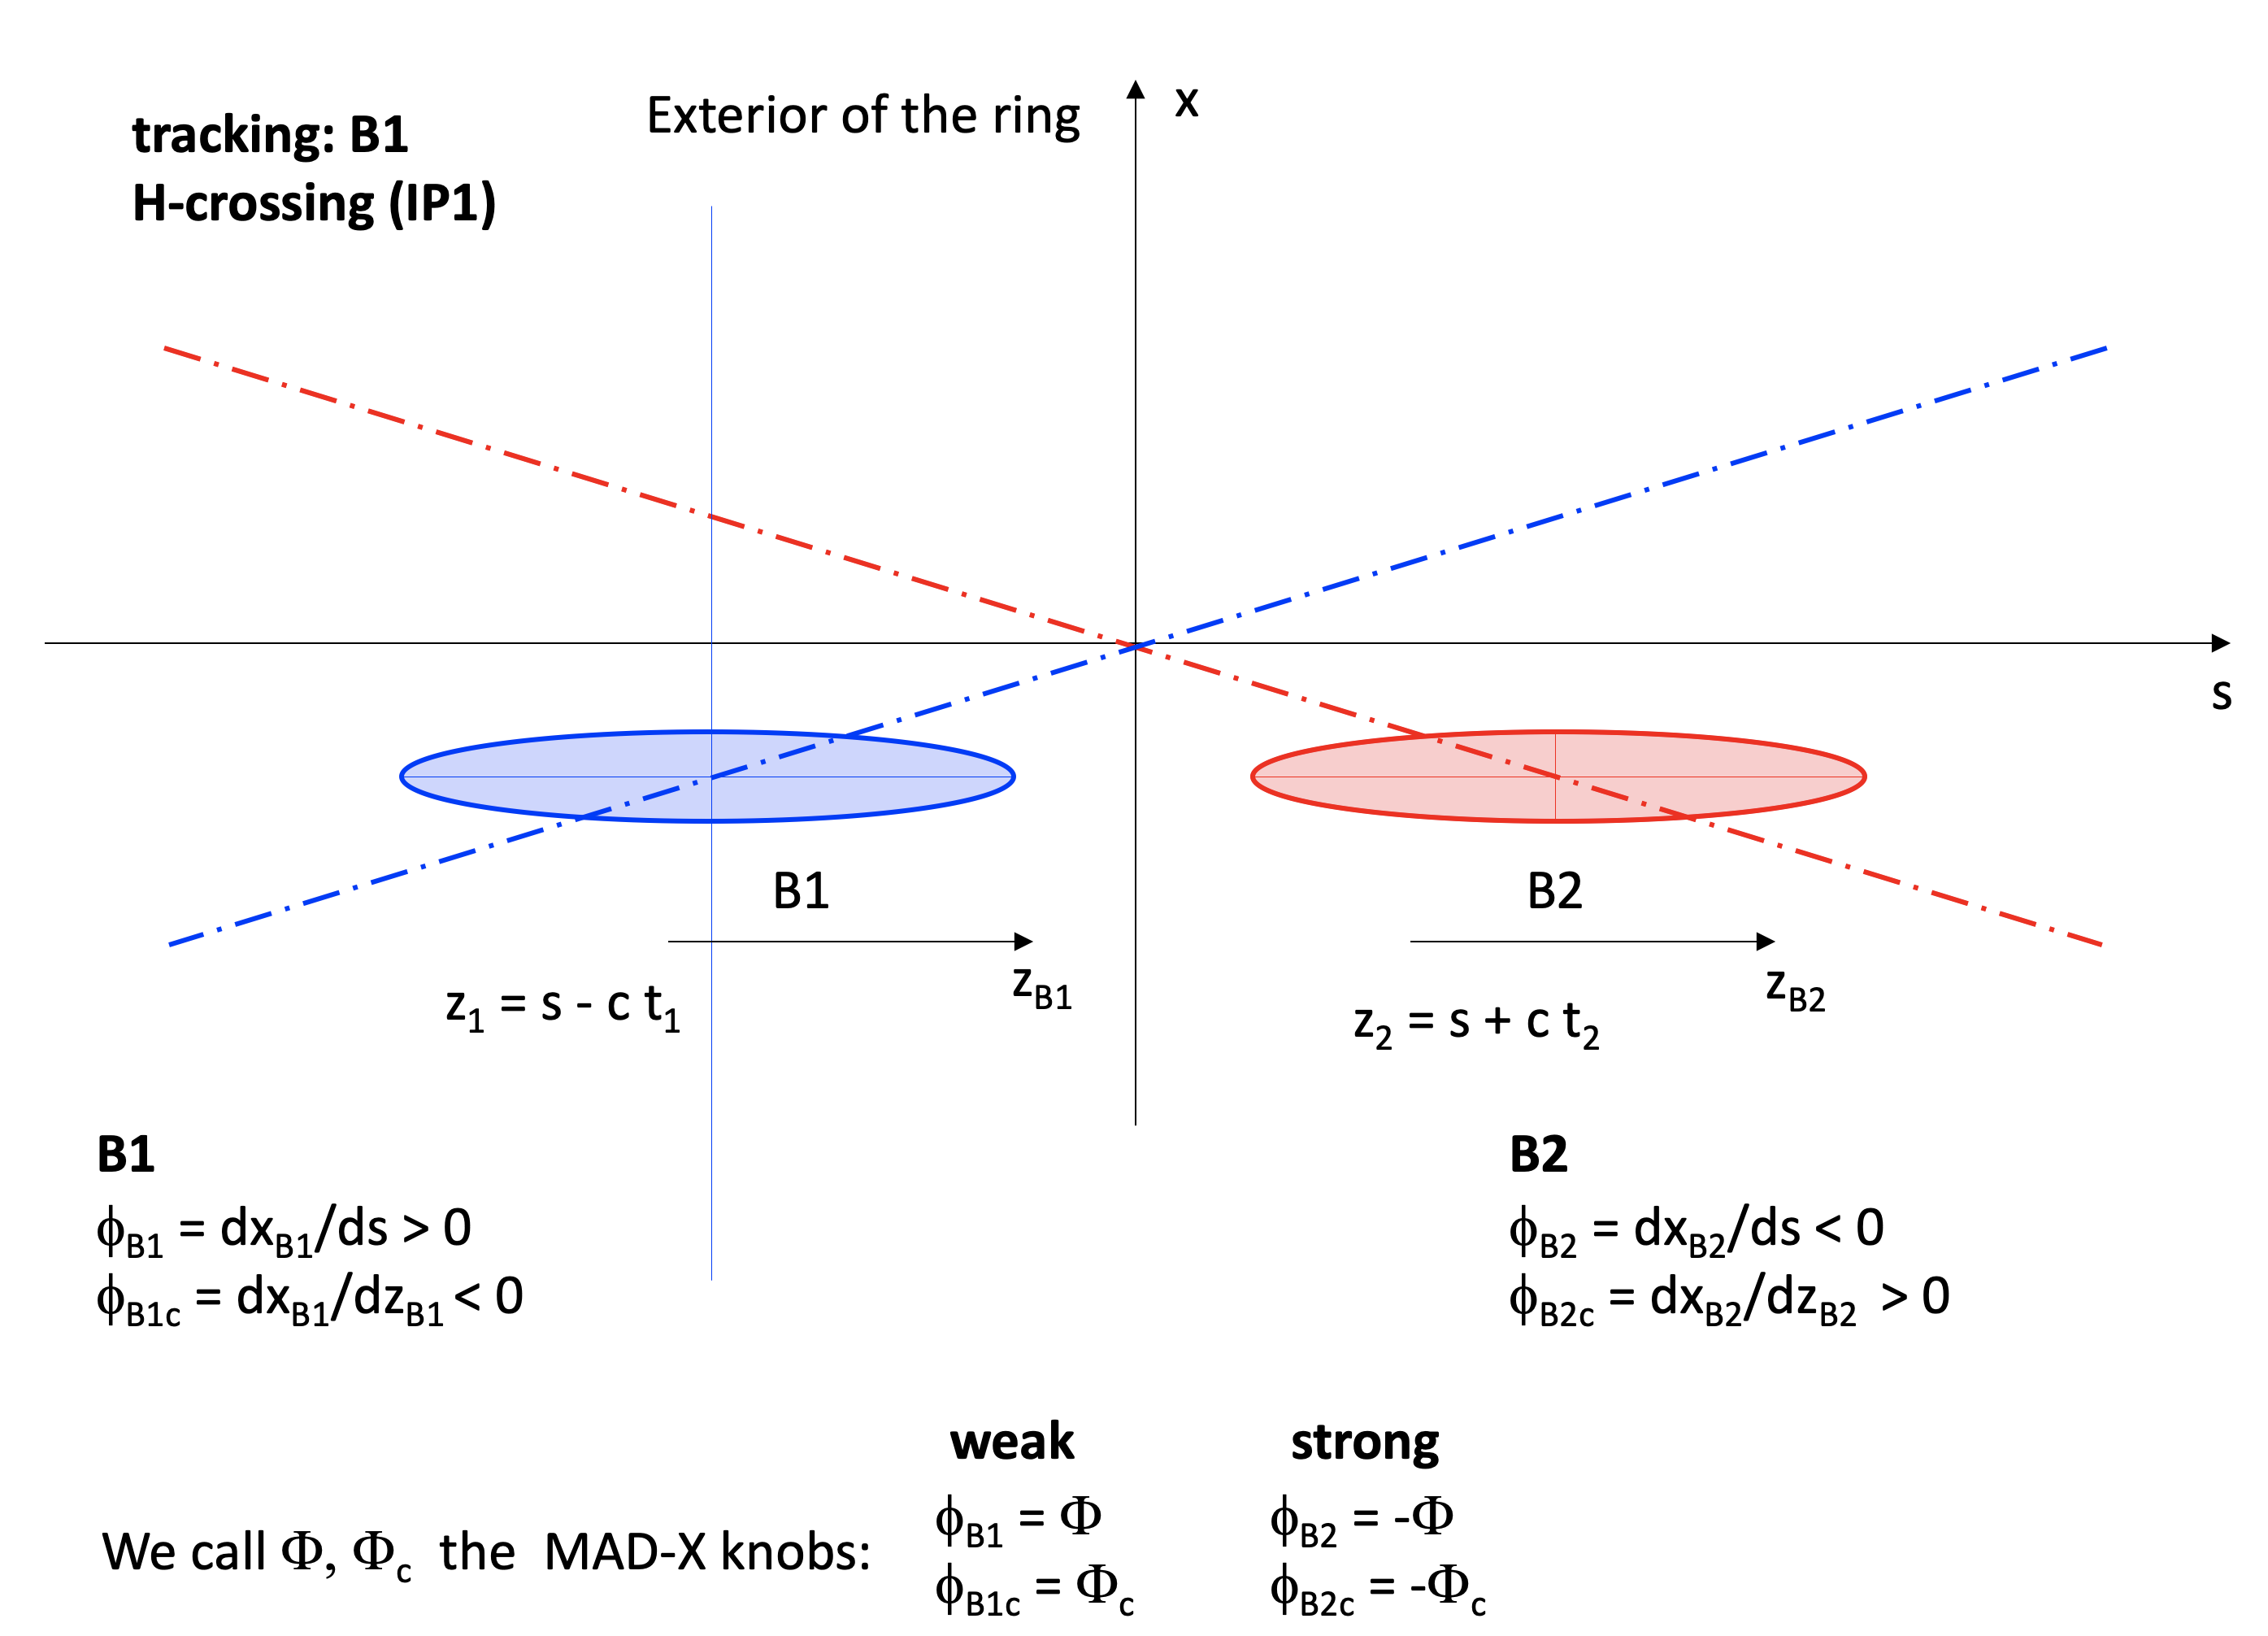
\includegraphics[width=.87\textwidth, trim=0cm 0cm 0cm 0cm, clip]{figures/b1ip1.png}
\caption{\small Crab crossing in the IP1 of the HL-LHC modeled for the tracking of the clockwise beam (beam~1).  \label{fig:crab_ip1b1}}
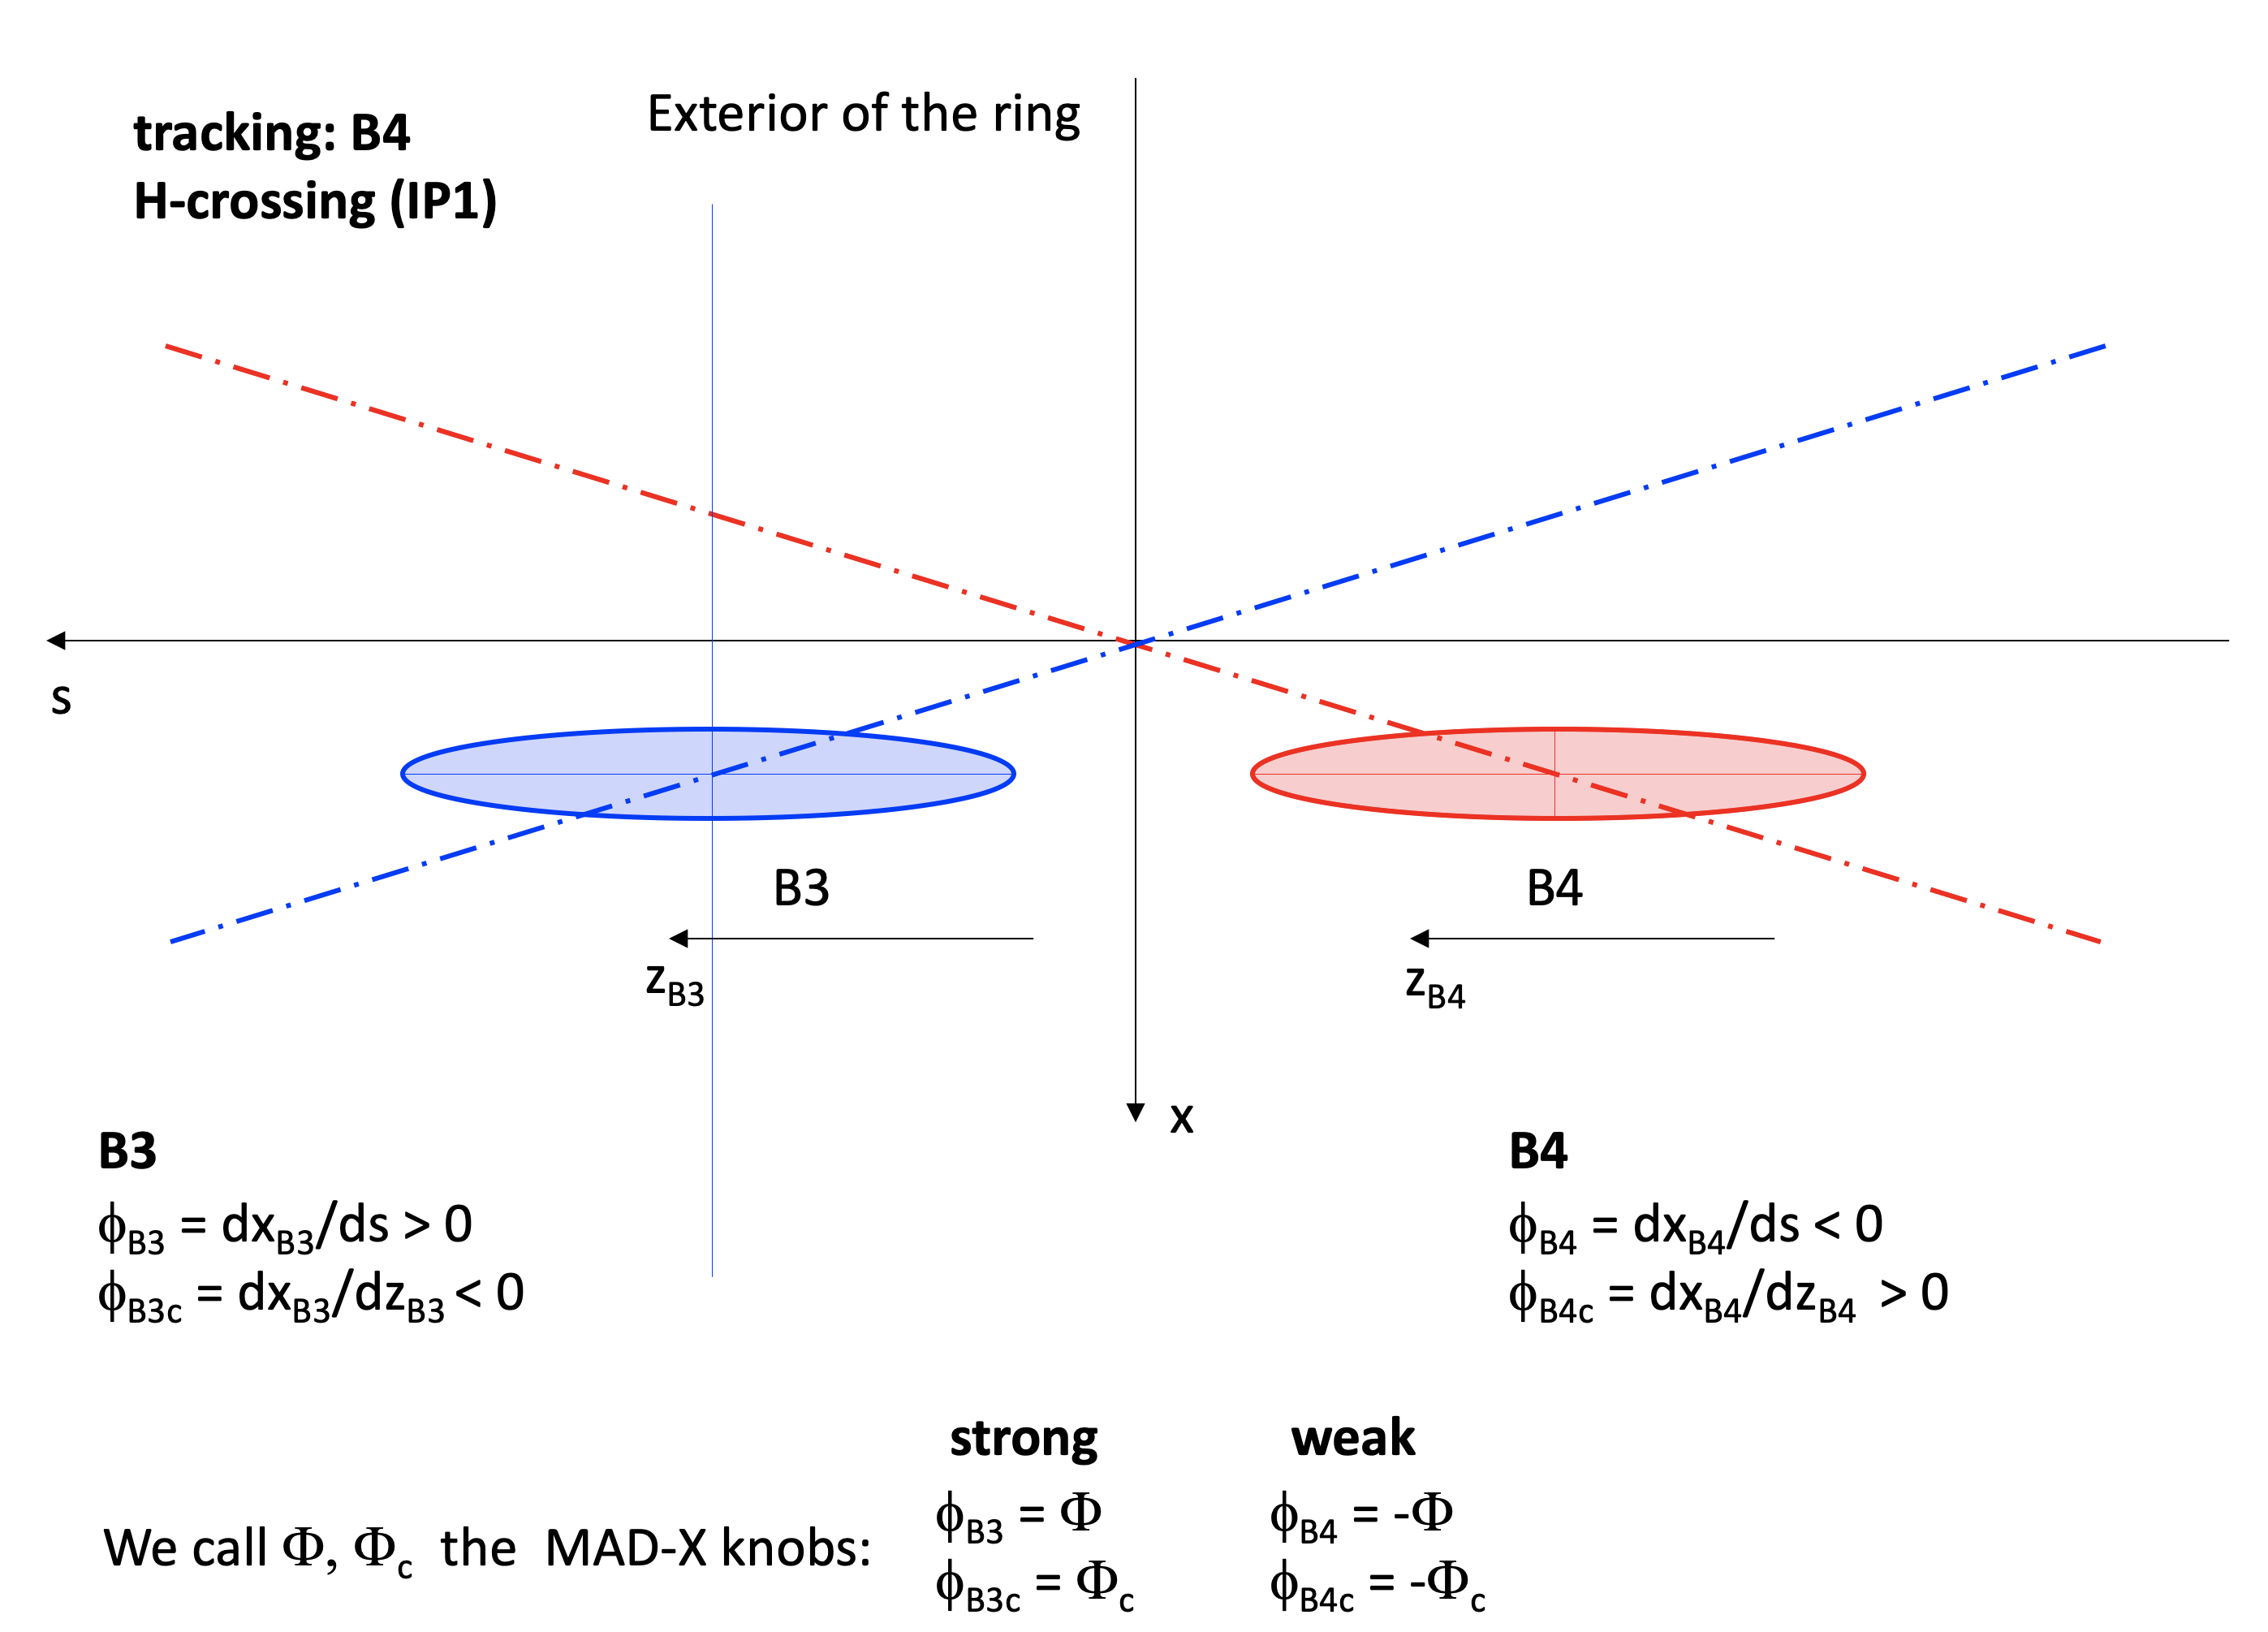
\includegraphics[width=.87\textwidth, trim=0cm 0cm 0cm 0cm, clip]{figures/b4ip1.png}
\caption{\small Crab crossing in the IP1 of the HL-LHC modeled for the tracking of the anticlockwise beam (beam~4). \label{fig:crab_ip1b4}}
\end{figure}

\begin{figure}[p]
\centering
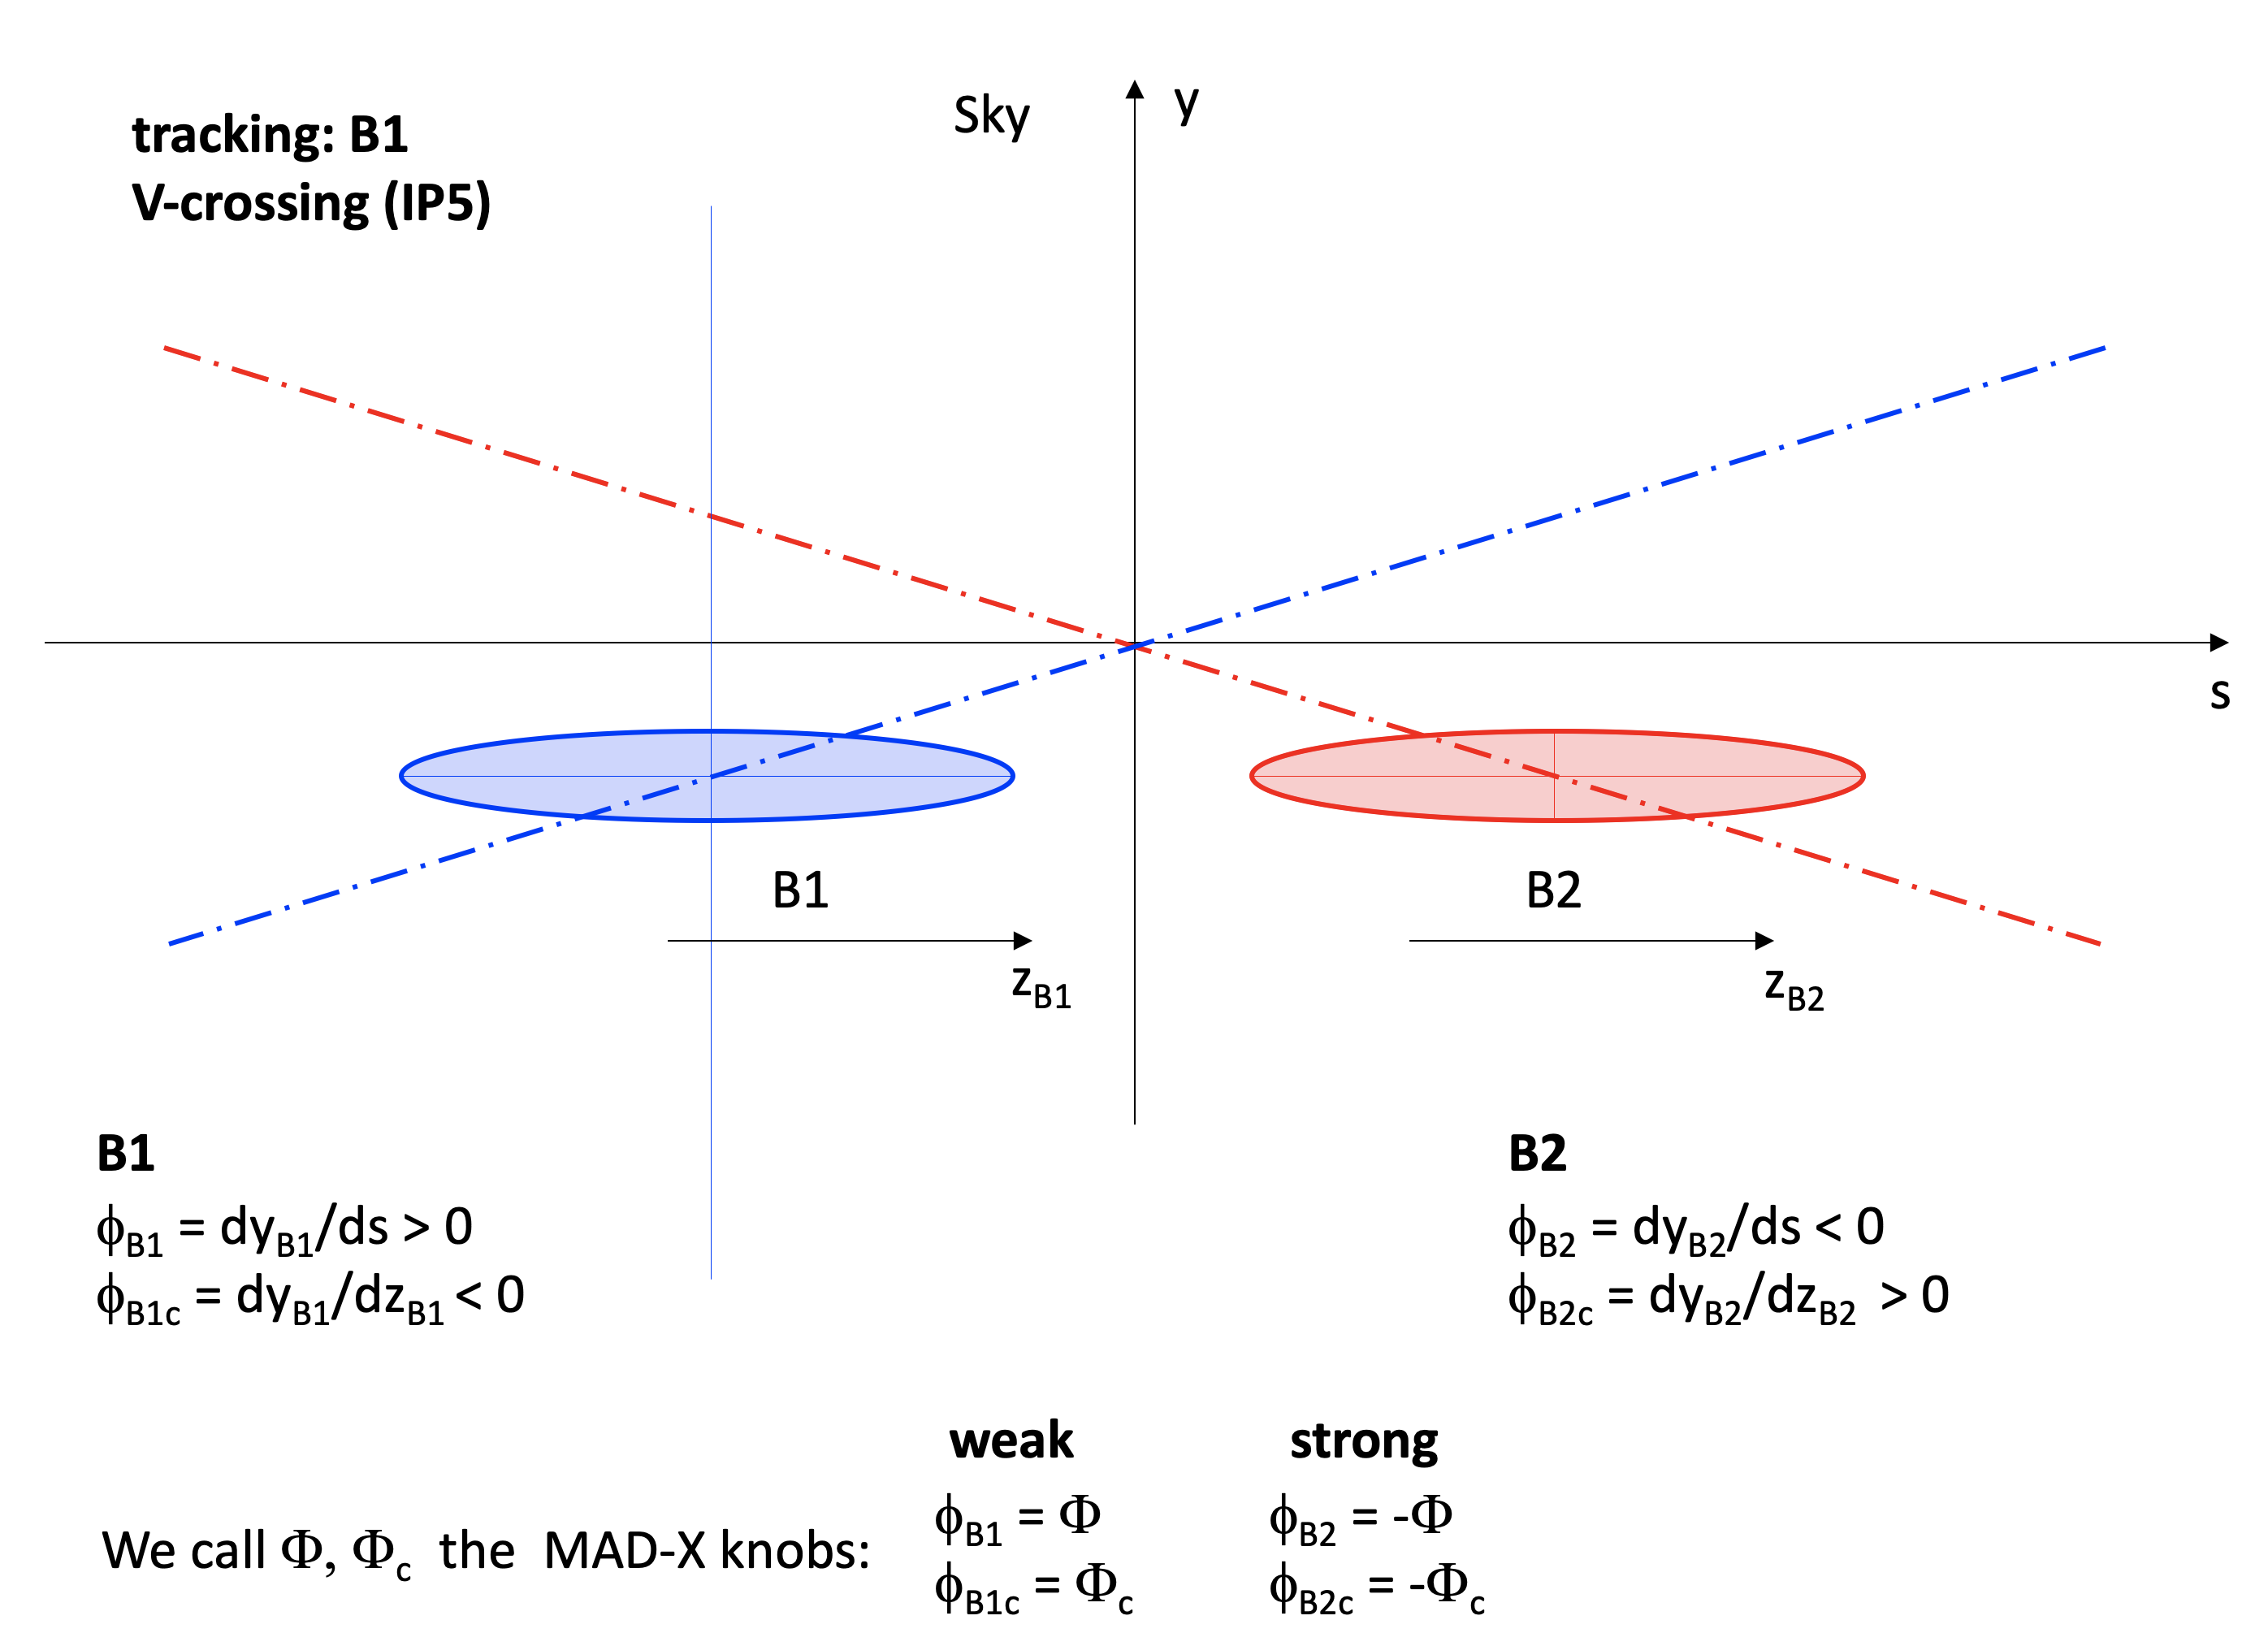
\includegraphics[width=.87\textwidth, trim=0cm 0cm 0cm 0cm, clip]{figures/b1ip5.png}
\caption{\small Crab crossing in the IP5 of the HL-LHC modeled for the tracking of the clockwise beam (beam~1).  \label{fig:crab_ip5b1}}
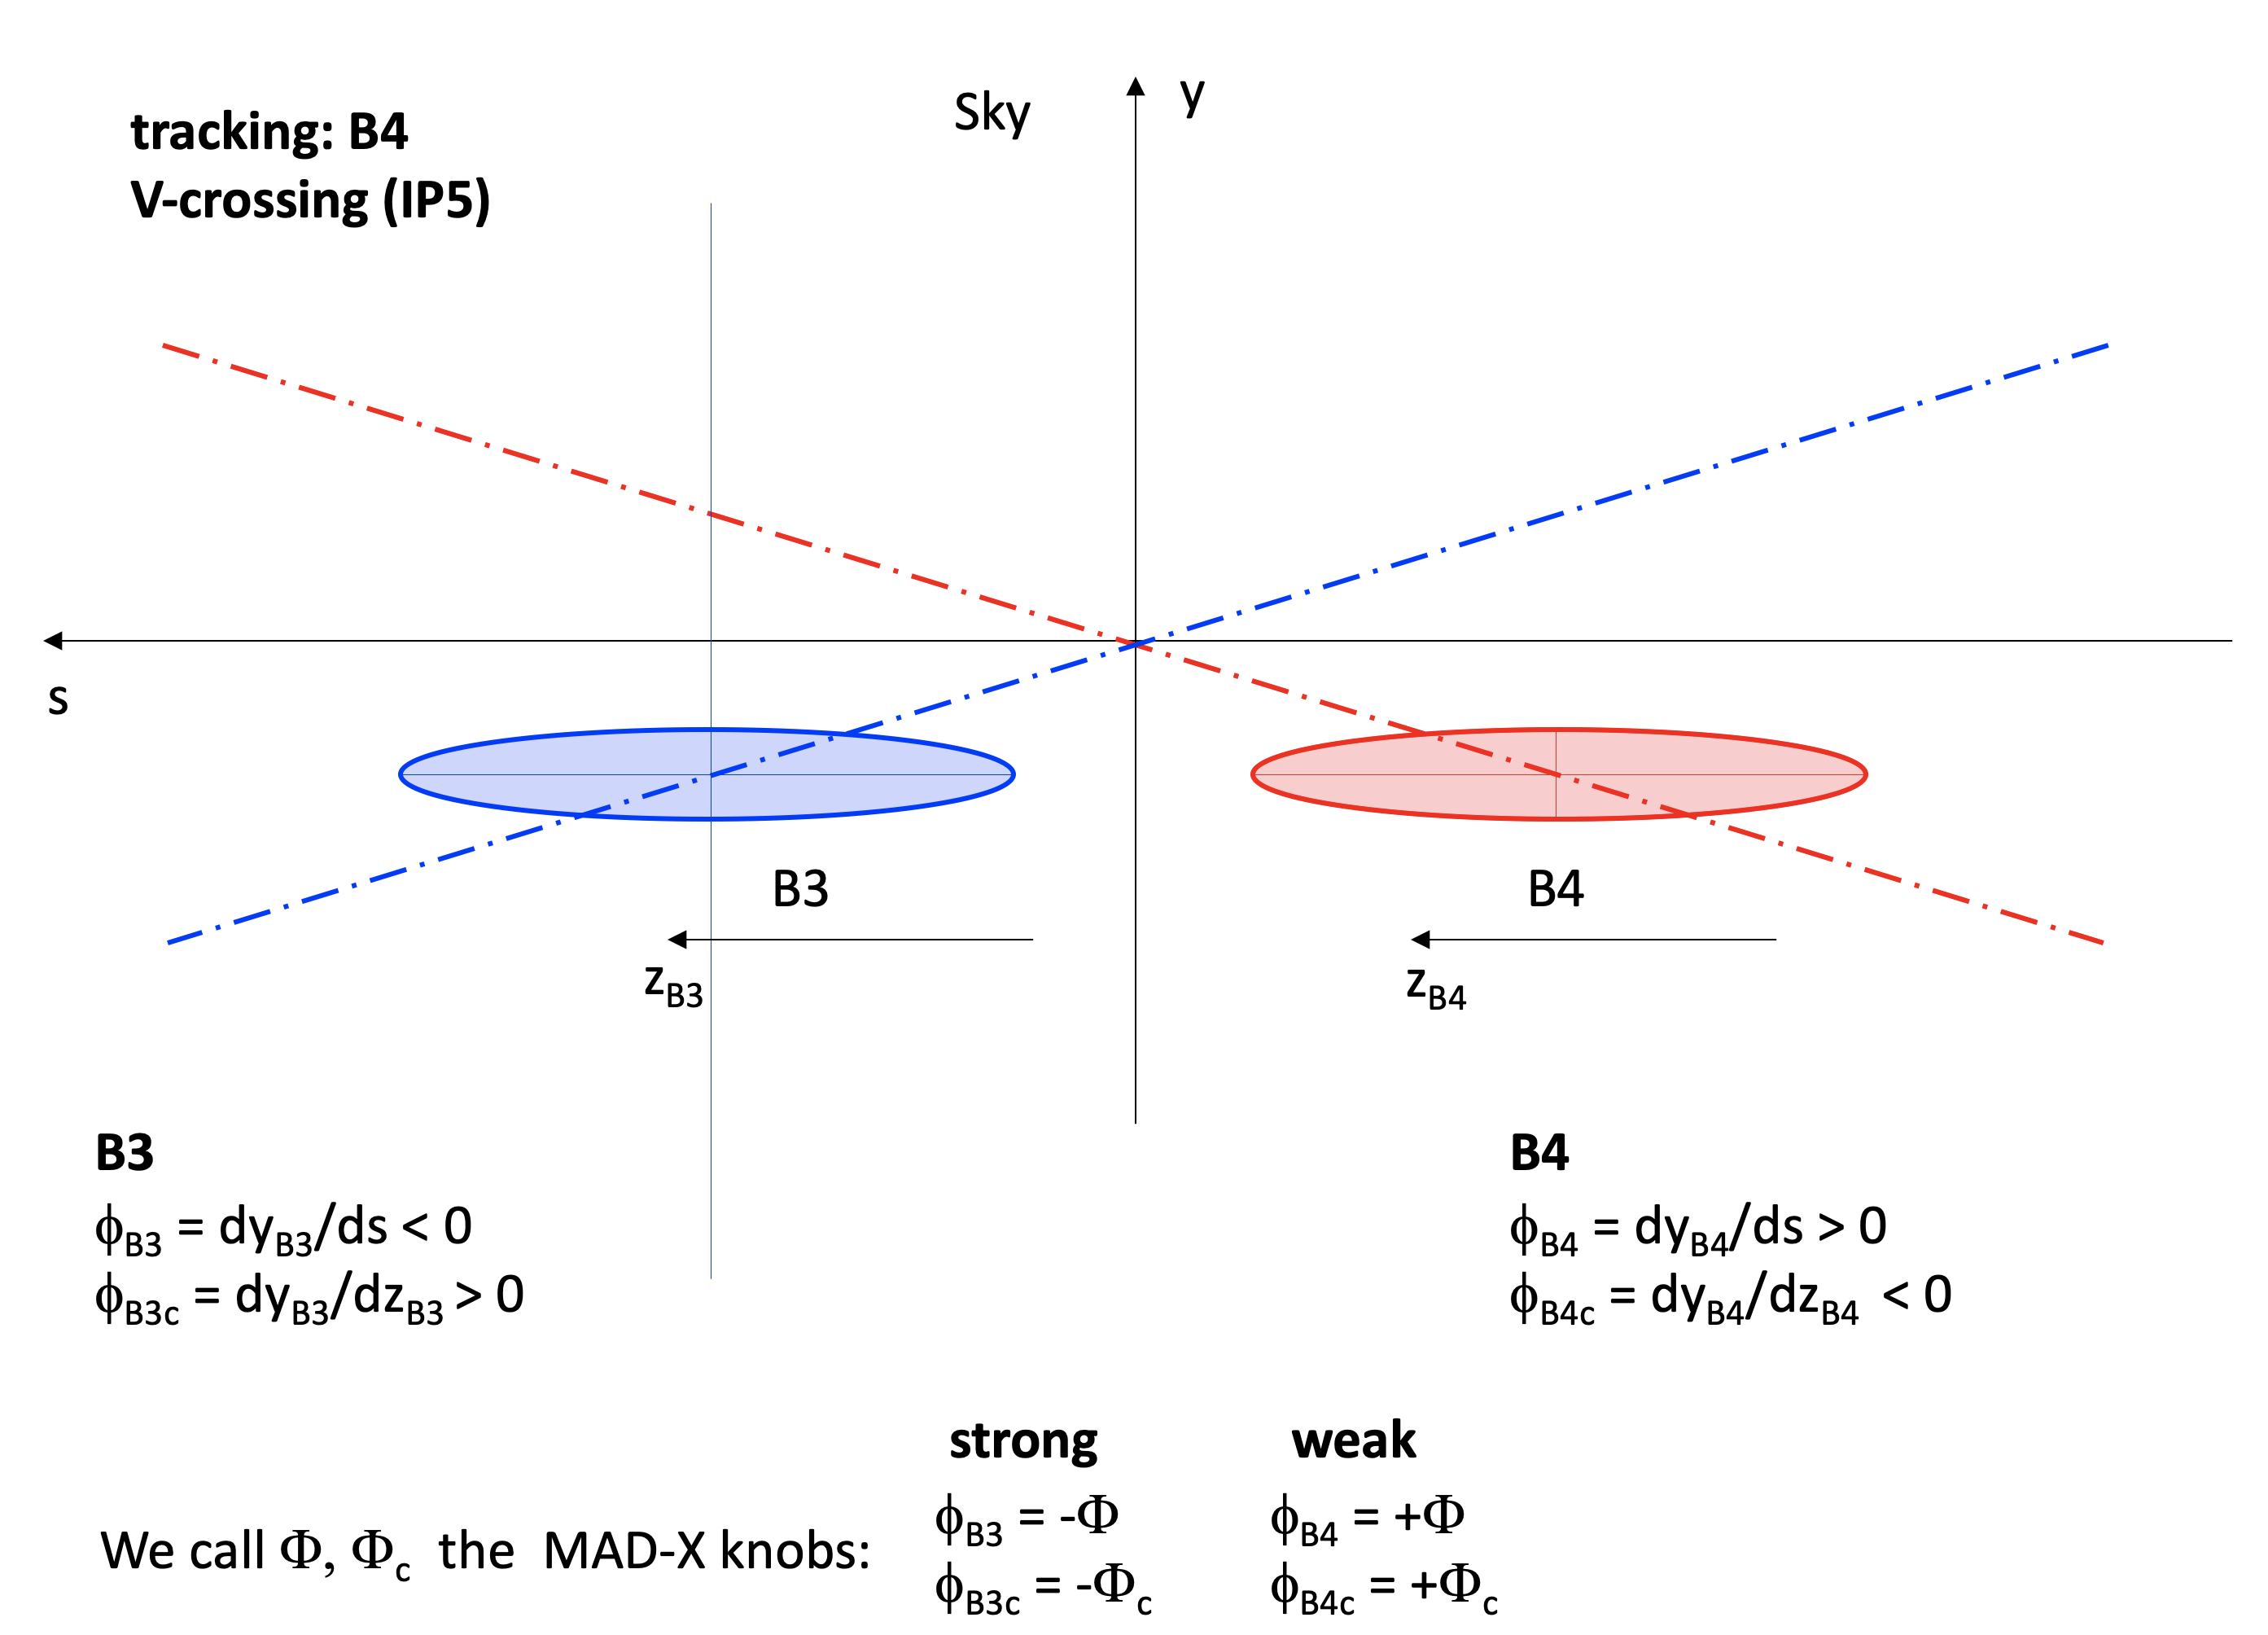
\includegraphics[width=.87\textwidth, trim=0cm 0cm 0cm 0cm, clip]{figures/b4ip5.png}
\caption{\small Crab crossing in the IP5 of the HL-LHC modeled for the tracking of the anticlockwise beam (beam~4). \label{fig:crab_ip5b4}}
\end{figure}

\subsection{Configuration of beam-beam lenses for beam 1}

In order to model the HO interaction for a crab crossing, the ``strong bunch'' is sliced longitudinally using the constant charge method, and one beam-beam lens for each slice is installed in the sequence.

In particular, in the sequence of beam 1, the lens corresponding to a slice of the strong beam (beam 2) having longitudinal coordinate $z_2=Z_2$ is installed at the location where the slice encounters the synchronous particle of the weak beam (see Eq.\,\eqref{eq:cp} with $z_1 = 0$):
\begin{equation}
    s_\text{lens} = +\frac{Z_2}{2}
    \, .
    \label{eq:slens}
\end{equation}


The position of the strong beam at the lens can be found replacing Eq.\,\eqref{eq:slens} into Eq.\,\eqref{eq:x2}:
\begin{equation}
   X_2 = - s_\text{lens} (\phi + 2 \phi_c)
   \, .
\end{equation}

The effect of the crab bump alone is given by:
\begin{equation}
   X^\text{crab}_2 = - 2 \phi_c s_\text{lens} = -\phi_c Z_2 \, .
\end{equation}

Taking into account the RF curvature coming from the crab cavity frequency, the position of the slice at the beam-beam lens can be written as:
\begin{equation}
   X^\text{crab}_2 = -\phi_c \frac{L_\text{ring}}{2 \pi h_\text{CC}} \sin\left(  \frac{2 \pi h_\text{CC}}{L_\text{ring}} Z_2\right) = -\phi_c \frac{L_\text{ring}}{2 \pi h_\text{CC}} \sin\left(  \frac{2 \pi h_\text{CC}}{L_\text{ring}} 2 s_\text{lens}\right)
   \, ,
   \label{eq:x2crab}
\end{equation}
where $h_\text{CC}$ is the harmonic number of the crab cavity and $L_\text{ring}$ is the circumference of the ring.

\subsection{Configuration of beam-beam lenses for beam 2}
In the sequence of beam 2, we install the beam-beam lens for a slice of the strong beam (beam 1) having longitudinal coordinate $z_1=Z_1$ at the location where the slice encounters the synchronous particle of the weak beam, (see Eq.\,\eqref{eq:cp} with $z_2 = 0$):
\begin{equation}
    s_\text{lens} = \frac{Z_1}{2}
    \, .
    \label{eq:slensb2}
\end{equation}

The position of the strong beam at the lens can be found replacing Eq.\,\eqref{eq:slensb2} into\,Eq.\,\eqref{eq:x1}:
\begin{equation}
   X_1 = s_\text{lens} (\phi + 2 \phi_c)
   \, .
\end{equation}

The effect of the crab bump alone is given by:
\begin{equation}
   X^\text{crab}_1 = 2 \phi_c s_\text{lens} = \phi_c Z_1
   \, .
\end{equation}

Taking into account the RF curvature coming from the crab cavity frequency, the position of the slice at the beam-beam lens can be written as:
\begin{equation}
   X^\text{crab}_1 = \phi_c \frac{L_\text{ring}}{2 \pi h_\text{CC}} \sin\left(  \frac{2 \pi h_\text{CC}}{L_\text{ring}} Z_1\right) = \phi_c \frac{L_\text{ring}}{2 \pi h_\text{CC}} \sin\left(  \frac{2 \pi h_\text{CC}}{L_\text{ring}} 2 s_\text{lens}\right)
   \, .
   \label{eq:x1crab}
\end{equation}

From Eqs.\,\eqref{eq:x2crab} and \eqref{eq:x1crab}, we find that for lenses at the same longitudinal position $s_\text{lens}$ the corresponding slices of the two beams $Z_1 = Z_2 = 2 s_\text{lens}$ have opposite transverse coordinates:
\begin{equation}
X^\text{crab}_1= -X^\text{crab}_2
\, .
\end{equation}

\subsection{Crab bump from MAD-X twiss}

For a non-ideal crabbing, for example in the presence of a non-closure of the crab-bump, the realistic $z$-dependent  orbit distortion introduced by the crab cavities can be characterized using the MAD-X twiss, by installing orbit correctors at the position of the crab cavities that introduce the crab cavity deflection as seen at a certain reference position along the bunch $z_\text{ref}$. 
To obtain the effect on particles at different positions along bunch it is possible to apply the following scaling:
\begin{equation}
x\left(z\right) = x\left(z_\text{ref}\right)
 \cfrac
 {\sin\left(  \frac{2 \pi h_\text{CC}}{L_\text{ring}} z\right)}
 {\sin\left(  \frac{2 \pi h_\text{CC}}{L_\text{ring}} z_\text{ref}\right)} 
 \, .
\end{equation}

\section{Step-by-step configuration procedure}

Based on the method introduced in the previous sections, the following procedure has been implemented in pymask to configure the beam-beam lenses in the sixtrack and sixtracklib tracking model:

\begin{enumerate}
\item Inactive beam-beam lenses (not configured) are installed in both clockwise sequences (Beam~1 and Beam~2) at the locations of the HO and LR beam-beam encounters. As discussed in Sec.\,\ref{sec:crab}, at each IP a set of lenses is installed to model the HO, one corresponding to each bunch slice.
\item The MAD-X twiss and survey tables are computed 
for both clockwise sequences.
\item The transverse beam shapes ($\Sigma$-matrix) are extracted from the twiss table for all beam-beam lenses.
\item The positions of the beams at the beam-beam lenses in the lab frame are computed combining the information from the survey and twiss tables, as discussed in Sec.\,\ref{sec:posdir}.
\item The beam-beam separations are computed, as discussed in Sec.\,\ref{sec:separ}.
\item For all HO interactions, the crossing plane and the crossing angle are identified, as discussed in Sec.\,\ref{sec:xing}.
\item The relevant quantities for the beam-beam lenses in the anticlockwise sequences (Beam~3 and Beam~4) are obtained from the data computed for the lenses in the clockwise sequences (Beam~1 and Beam~2), using the transformations described in Sec.\,\ref{sec:b4}.
\item The effect of the crab cavities is introduced by using the shape of the crab bumps obtained from twiss tables computed with orbit correctors at the locations of the cavities, as discussed in Sec.\,\ref{sec:crab}.
\item The information computed before is used to configure the beam-beam lenses in the MAD-X model of the sequence for which the tracking simulation will be performed, typically either Beam 1 or Beam 4.
\item The SixTrack input and the pysixtrack/sixtracklib input files are generated  using the MAD-X model and the additional information computed as described above. 
\item The closed orbit as computed from the MAD-X sequences is saved on file, for the generation of matched beam distributions and for the computation of the beam-beam dipolar kicks on the closed orbit, which are usually subtracted in weak-strong tracking simulations.


\end{enumerate}


\section*{Acknowledgments}
The authors would like to thank all the colleagues who  have contributed to the development of the MAD-X tools for the configuration of tracking simulations, on which the present work is largely based, and have provided important input and support, in particular G.~Arduini, J.~Barranco~Garcia, R.~De~Maria, S.~Fartoukh, M.~Giovannozzi, S.~Kostoglou, E.~M\'etral,  Y.~Papaphippou, D.~Pellegrini, T.~Pieloni and F.~Van Der Veken.